\documentclass{article}[12pt]
\usepackage[utf8]{inputenc}
\usepackage{tikz}
\usepackage{color}
\usepackage{subfiles}
\usepackage[T1]{fontenc}
\usepackage{titlepic}
\usepackage{subfiles}
\usepackage{amssymb}
\graphicspath{ {figures/} }
\usepackage{array}
\usepackage{graphicx}
\usepackage{float}
\usepackage{caption}
\usepackage{subcaption}
\usepackage{amsmath}
\usepackage{algorithm2e}
\usepackage{algorithmic}
\usepackage{forest}
\usepackage{commath}
\usepackage{pdfpages}
\usepackage[section]{placeins}
\usepackage{hyperref}

\hypersetup{
	colorlinks,
	citecolor=violet,
	linkcolor=blue,
	urlcolor=blue}



\title{\Huge{NS3 Project Report}}
\author{\textbf{Sihat Afnan} \\
        \textbf{Student Id. : 1705098} 
     }
\date{\large February , 2022}


\begin{document}

\maketitle

\vspace{4cm}

\begin{figure}[h!]
\centering
    
\includegraphics[width = 0.25\textwidth]{Pictures/logoBUET.png}
\end{figure}
\begin{center}
\vspace{.5cm}

\Large{Department of Computer Science and Engineering \\
    Bangladesh University of Engineering and Technology \\
    (BUET) \\
    Dhaka - 1000 }

\end{center}
\newpage

\tableofcontents
\newpage

\listoffigures
\newpage

\section{Introduction}
    NS3 is an open-source event-driven simulator designed specifically for research in computer communication networks. In this project, I have to vary different parameters such as number of nodes, number of flows, number of packets per second and measure some metrics and plot them in some graphs. \\
    I also had to modify some mechanisms of Retransmission Timeout calculation and compare the modified version with the original implementation of NS3.The paper from which I have taken idea from is
    \begingroup
    \hypersetup{hidelinks}
    \href{http://citeseerx.ist.psu.edu/viewdoc/download?doi=10.1.1.76.2748&rep=rep1&type=pdf}{\textcolor{blue}{The Peak-Hopper: A New End-to-End
    	Retransmission Timer for Reliable Unicast Transport} }
    \endgroup 
    
  
    
\section{Simulated Networks}
\begin{itemize}
    \item Wireless 802.11 (static) network using AODV routing in Random topology
    \item Wireless 802.15.4 (static) network using Ripng routing in Random Topology
    \item Dumbbell topology consisting of same number of senders and receivers and two routers for showing RTT and RTO modification.
  
\end{itemize}
    
\section{Parameters and Metrics}
    \subsection{Parameters}
        \begin{enumerate}
            \item Number of nodes (20, 40, 60, 80, and 100)
            \item Number of flows  (10, 20, 30, 40, and 50)
            \item Number of packets per second  (10, 20, 30, 40, and 50)
            \item Coverage Area (1000 , 1500 , 2000 , 2500  ,2800 $m^2$) 
        \end{enumerate}

    \subsection{Metrics}
        \begin{enumerate}
            \item Network Throughput
            \item End-to-End Delay
            \item Packet Delivery Ratio 
            \item Packet Drop Ratio
        \end{enumerate}


\section{Overview of the proposed algorithm}
The PeakHopper algorithm essentially runs two RTO algorithms in parallel.One algorithm (Short-Term History RTO) monitors the present and short-term history in order to respond to RTT increases. The other algorithm(Long-Term History RTO) simply decays the current value of RTO, and can therefore be said to represent the long-term history.\\

\begin{figure}[!h]
	\centering
	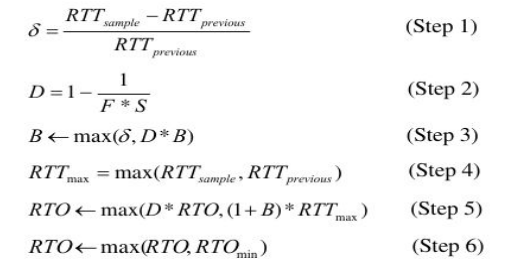
\includegraphics[width=.9\textwidth]{Pictures/algo/algo.png}
	\caption{Algorithm Overview}
\end{figure}

   \begin{enumerate}
	\item Having collected a new RTT sample, RTTsample,
	we compare this value to the previous RTT
	sample collected, RTTprevious, as shown in Step
	1. We call the normalized change between these
	two samples delta. This is the measure of the
	short-term changes in RTT.
	\item In Step 2, we further define a decay factor, D. D
	determines how rapidly the RTO is decayed. We
	also introduce a fader variable, F, which controls
	the speed of this decay (a high F gives a slow
	decay and vice versa).
	\item In Step 3, we calculate a booster variable B.
	The booster variable determines how high the
	RTO should hop when a large RTT increase
	has been detected.
	\item  In Step 4, we set RTTmax to the maximum of
	the new RTT sample, RTTsample, and the
	previous RTT sample, RTTprevious. RTTmax is
	used to represent the short-term history of the
	RTT.
	\item  In step 5, We set RTO to the maximum of a
	long-term history (represented by the term
	D*RTO ) and the short-term history
	(represented by the term ((1+B)*RTTmax).
	\item  In final step (Step 6), we ensure that the RTO
	does not fall below the minimum allowed RTO.
\end{enumerate}

\textbf{Metrics used in the paper}

\begin{figure}[!h]
	\centering
	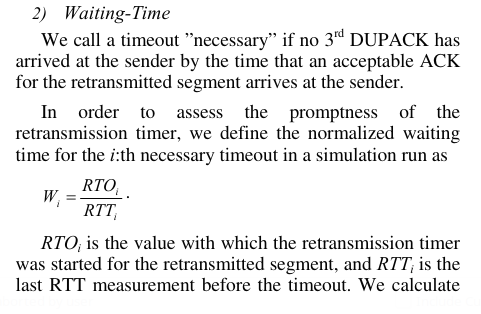
\includegraphics[width=.9\textwidth]{Pictures/algo/algo2.png}
	\caption{Metric 1}
\end{figure}

\begin{figure}[t!]
	\centering
	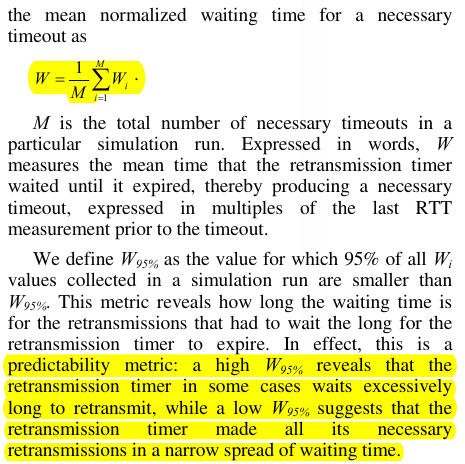
\includegraphics[width=.9\textwidth]{Pictures/algo/algo3.png}
	\caption{Metric 1}
\end{figure}

\begin{figure}[!h]
	\centering
	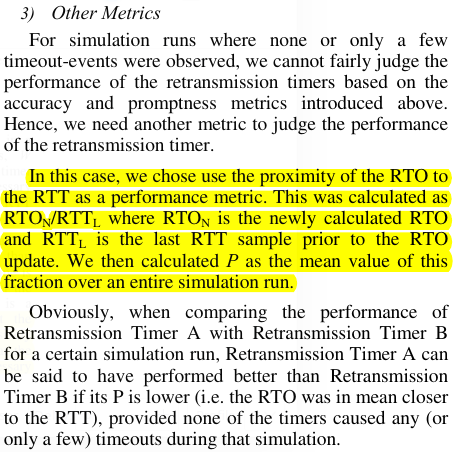
\includegraphics[width=.9\textwidth]{Pictures/algo/algo4.png}
	\caption{Metric 2}
\end{figure}




\section{Modifications}
\label{sec:mod}
    I have modified the RTT and RTO calculation algorithm in NS3.The relevant files were \textcolor{blue}{rtt-estimator.cc , rtt-estimator.h , tcp-socket-base.cc , tcp-socket-base.h }
    Apart from these , I have written a simulation script \textcolor{blue}{simulate.cc} to generate the topology and run my modified algorithm upon it.
    \begin{description}
        \item[\textbf{1. rtt-estimator.cc:}]
        
        Inside \textcolor{blue}{RttMeanDeviation::Measurement (Time m)} function,\\
		\begin{figure}[H]
			\centering
			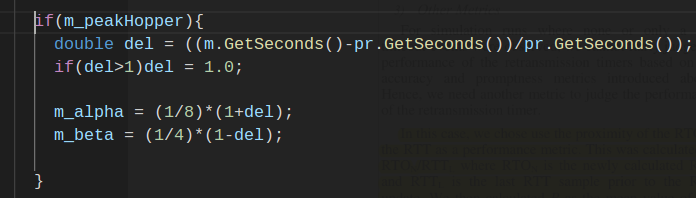
\includegraphics[width=.9\textwidth]{Pictures/algo/rtt_estimator2.png}
			\caption{rtt-estimator.c modification}
		\end{figure}   

    \item[\textbf{2. tcp-socket-base.h}]
    Declared necessary flag and trace values for calculation of metrics proposed in the paper.\\
    	\begin{figure}[H]
    	\centering
    	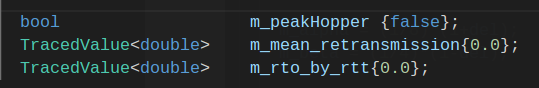
\includegraphics[width=.9\textwidth]{Pictures/algo/tcp-socket-base.h.png}
    	\caption{tcp-socket-base.h modification}
        \end{figure}   
    
    
    \item[\textbf{2. tcp-socket-base.cc}] 
    There are several modifications in this file.Following are the added attributes and trace sources added in tcp-socket-base class.\\
    
    \begin{figure}[H]
    	\centering
    	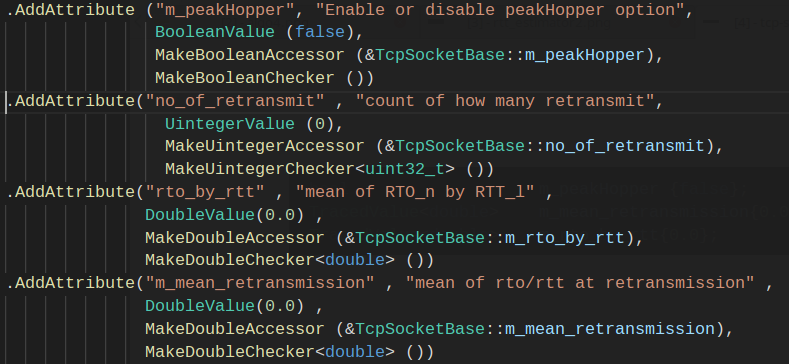
\includegraphics[width=.9\textwidth]{Pictures/algo/tcp-socket-base1.png}
    	\caption{Added attributes}
    \end{figure}   
    
	\begin{figure}[H]
		\centering
		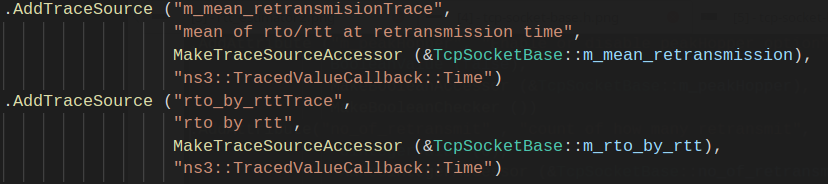
\includegraphics[width=.9\textwidth]{Pictures/algo/tcp-socket-base2.png}
		\caption{Added trace sources}
	\end{figure}   
	    
    In the \textcolor{blue}{TcpSocketBase::EstimateRtt (const TcpHeader tcpHeader)} function , following modification has been made when peakHopper flag is enabled
    
    \begin{figure}[H]
    	\centering
    	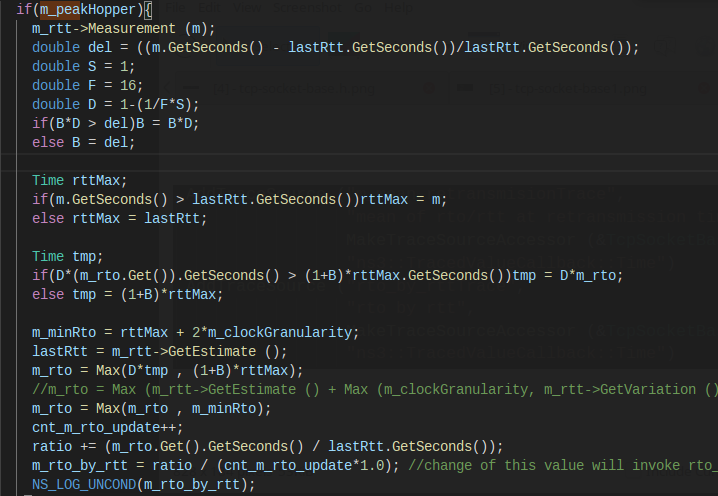
\includegraphics[width=.9\textwidth]{Pictures/algo/tcp-socket-base3.png}
    	\caption{estimateRtt method modification}
    \end{figure}   
    
    The next piece of modification is common for both \textcolor{blue}{TcpSocketBase::NewAck (SequenceNumber32 const ack, bool resetRTO)} and \textcolor{blue}{TcpSocketBase::SendEmptyPacket (uint8\_t flags)} functions.
    
    \begin{figure}[H]
    	\centering
    	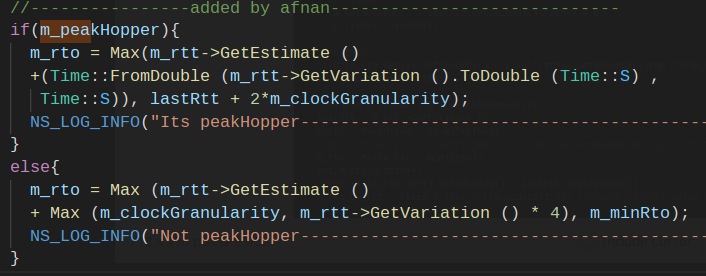
\includegraphics[width=.9\textwidth]{Pictures/algo/tcp-socket-base4.png}
    	\caption{NewAck and SendEmptypacket method modification}
    \end{figure}   
    
    \newpage
    
    Following modification was done in \textcolor{blue}{TcpSocketBase::DoPeerClose (void)} function while updating the lastRtt value\\
    
    \begin{figure}[H]
    	\centering
    	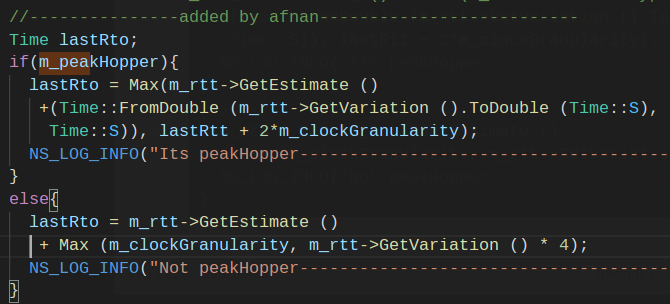
\includegraphics[width=.9\textwidth]{Pictures/algo/tcp-socket-base5.png}
    	\caption{DoPeerClose method modification}
    \end{figure}   
    
  Finally to calculate mean retransmission , following piece of code was added at the end of \textcolor{blue}{DoRetransmit()} function.
    
    \begin{figure}[H]
    	\centering
    	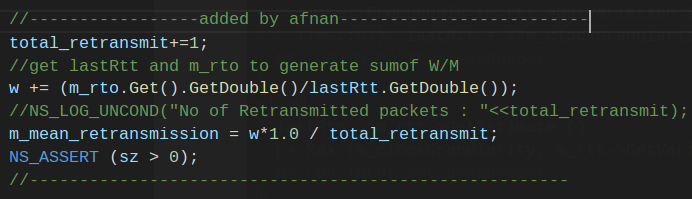
\includegraphics[width=.9\textwidth]{Pictures/algo/tcp-socket-base6.png}
    	\caption{mean retransmission calculation}
    \end{figure}   
    
    
    
    
    \end{description}
\newpage
\section{Comparison}
\subsection{RTT RTO modification}
\textbf{Network Topology Recap}
    \begin{figure}[H]
	\centering
	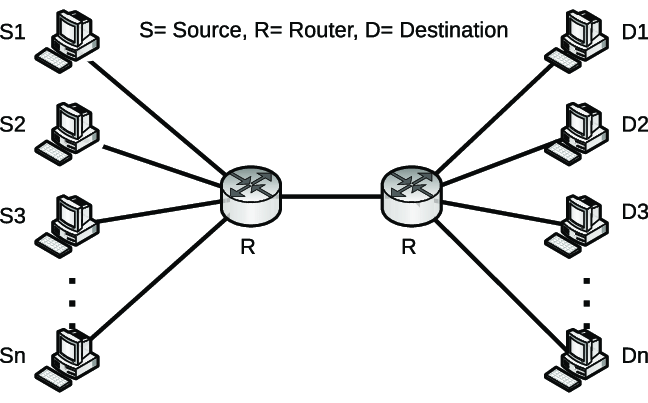
\includegraphics[width=\textwidth]{Pictures/dumbel.png}
	\caption{DumbBell Topology}
\end{figure}   

\newpage

\subsubsection{Access delay of 130ms and 45ms , shared delay 35ms }

\textbf{RTT and RTO }
    \begin{figure}[H]
	\centering
	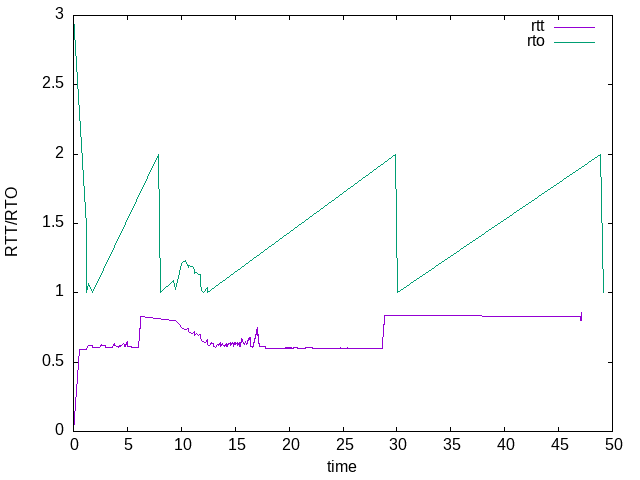
\includegraphics[height=0.6\textwidth]{Pictures/rtt/130/b/rtt_rto_graph.png}
	\caption{Default RTT RTO graph}
\end{figure}   

    \begin{figure}[H]
	\centering
	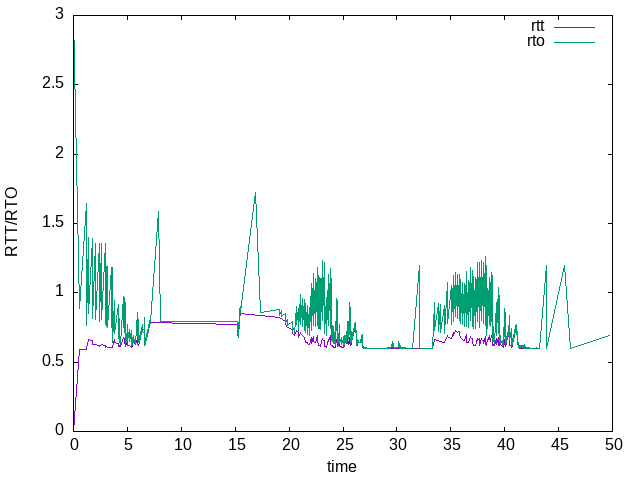
\includegraphics[height=.6\textwidth]{Pictures/rtt/130/m/rtt_rto_graph.png}
	\caption{Modified RTT RTO graph}
\end{figure}   

\newpage
\textbf{Mean Retransmission}
 \begin{figure}[H]
	\centering
	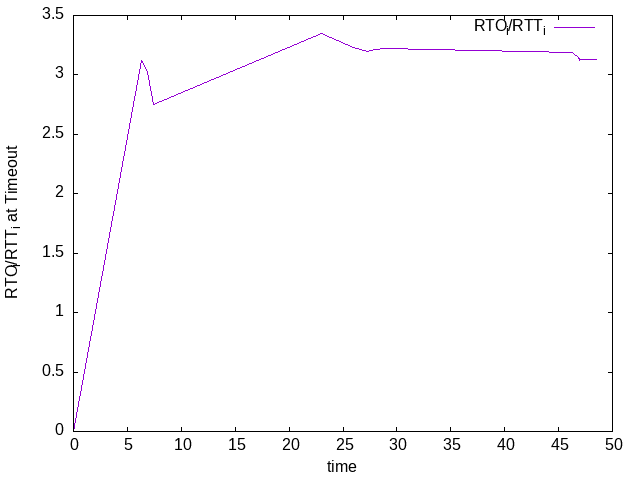
\includegraphics[height=0.6\textwidth]{Pictures/rtt/130/b/mean_retransmission.png}
	\caption{Default mean retransmission graph}
\end{figure}   

\begin{figure}[H]
	\centering
	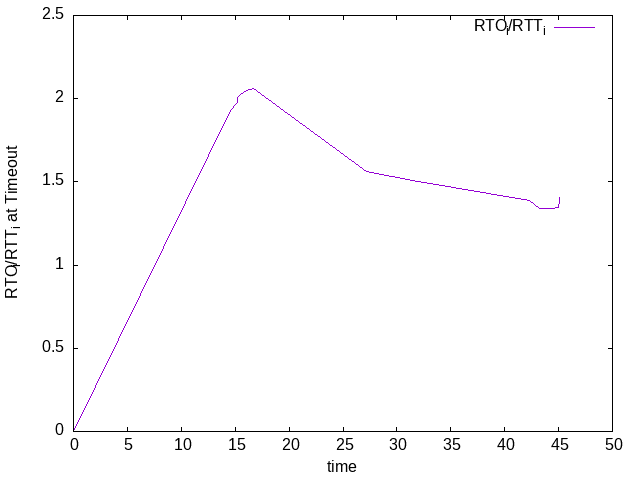
\includegraphics[height=.6\textwidth]{Pictures/rtt/130/m/mean_retransmission.png}
	\caption{Modified mean retransmission graph}
\end{figure}   

\newpage
\textbf{$RTO_i/RTT_i $ ratio}
\begin{figure}[H]
	\centering
	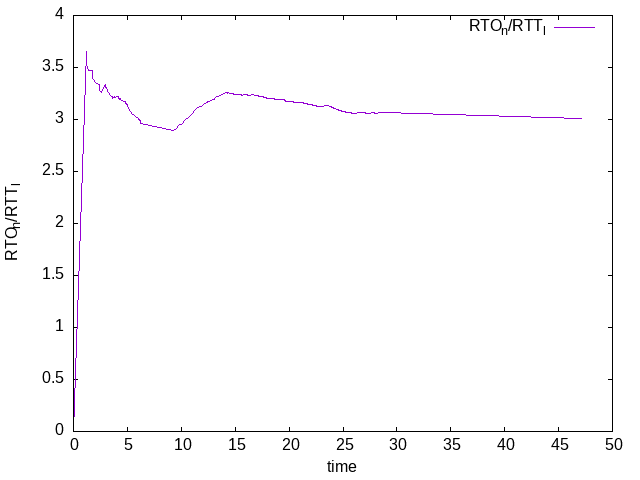
\includegraphics[height=0.6\textwidth]{Pictures/rtt/130/b/rto_by_rtt.png}
	\caption{Default rto/rtt graph}
\end{figure}   

\begin{figure}[H]
	\centering
	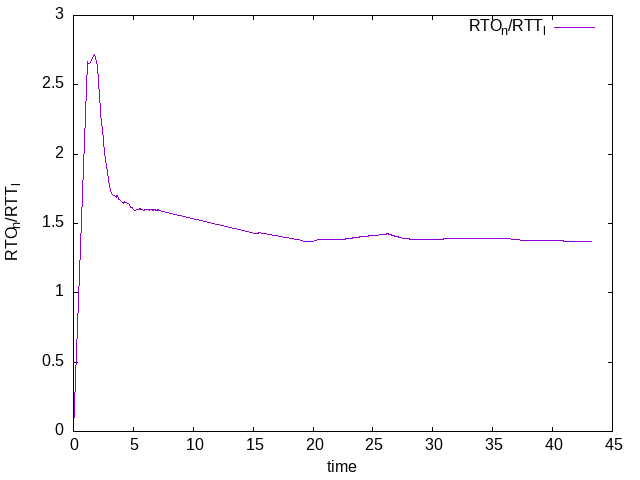
\includegraphics[height=0.6\textwidth]{Pictures/rtt/130/m/rto_by_rtt.png}
	\caption{Modified rto/rtt graph}
\end{figure}   

\newpage
\textbf{Congestion Window}
\begin{figure}[H]
	\centering
	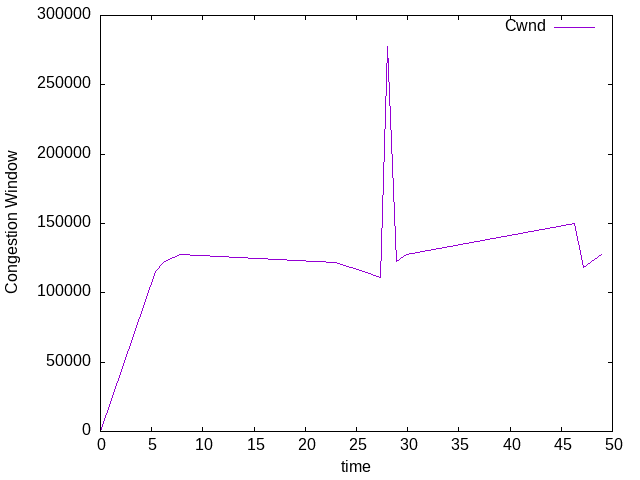
\includegraphics[height=0.6\textwidth]{Pictures/rtt/130/b/cwnd_graph.png}
	\caption{Default cwnd graph}
\end{figure}   

\begin{figure}[H]
	\centering
	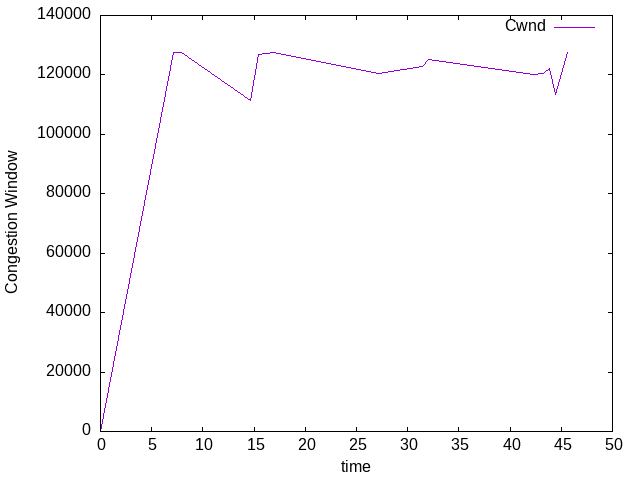
\includegraphics[height=0.6\textwidth]{Pictures/rtt/130/m/cwnd_graph.png}
	\caption{Modified cwnd graph}
\end{figure}   

\newpage
\textbf{Slow Start Threshold}
\begin{figure}[H]
	\centering
	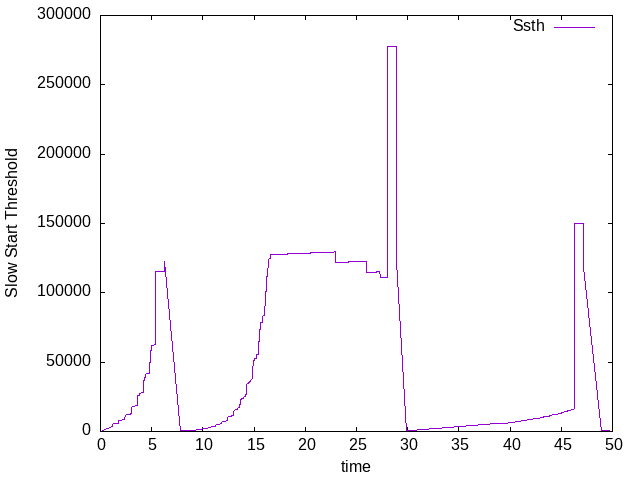
\includegraphics[height=0.6\textwidth]{Pictures/rtt/130/b/ssth_graph.png}
	\caption{Default ssth graph}
\end{figure}   


\begin{figure}[H]
	\centering
	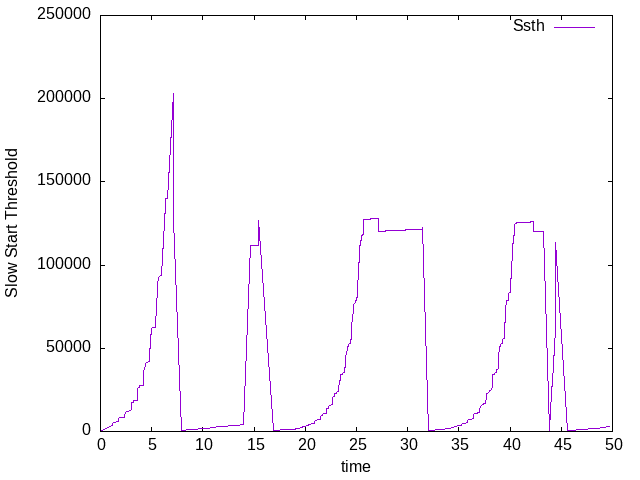
\includegraphics[height=0.6\textwidth]{Pictures/rtt/130/m/ssth_graph.png}
	\caption{Modified ssth graph}
\end{figure}   


\newpage
\subsubsection{access delay of 140 ms and 50 ms, shared delay 40 ms}


\textbf{RTT and RTO }
\begin{figure}[H]
	\centering
	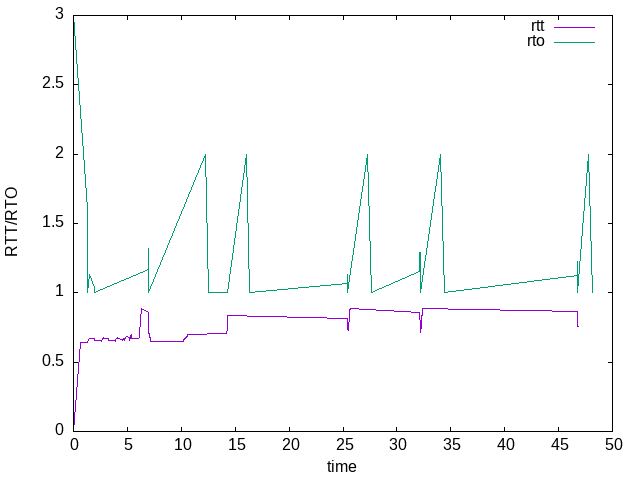
\includegraphics[height=0.6\textwidth]{Pictures/rtt/175/b/rtt_rto_graph.png}
	\caption{Default RTT RTO graph}
\end{figure}   

\begin{figure}[H]
	\centering
	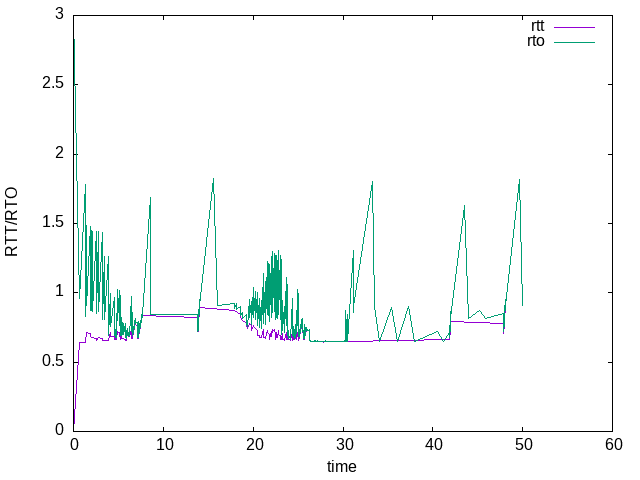
\includegraphics[height=.6\textwidth]{Pictures/rtt/175/m/rtt_rto_graph.png}
	\caption{Modified RTT RTO graph}
\end{figure}   

\newpage
\textbf{Mean Retransmission}
\begin{figure}[H]
	\centering
	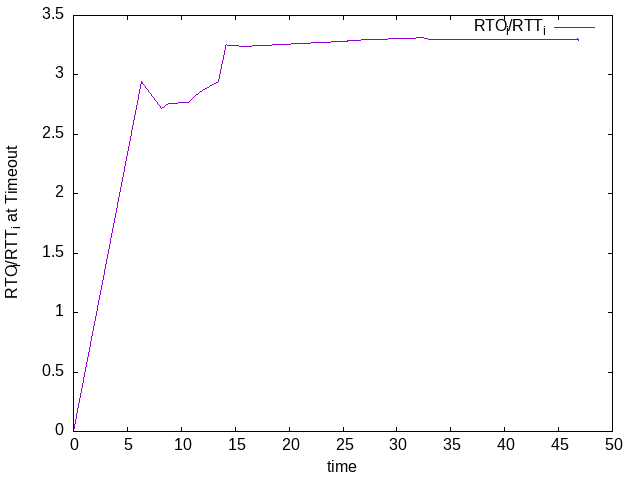
\includegraphics[height=0.6\textwidth]{Pictures/rtt/175/b/mean_retransmission.png}
	\caption{Default mean retransmission graph}
\end{figure}   

\begin{figure}[H]
	\centering
	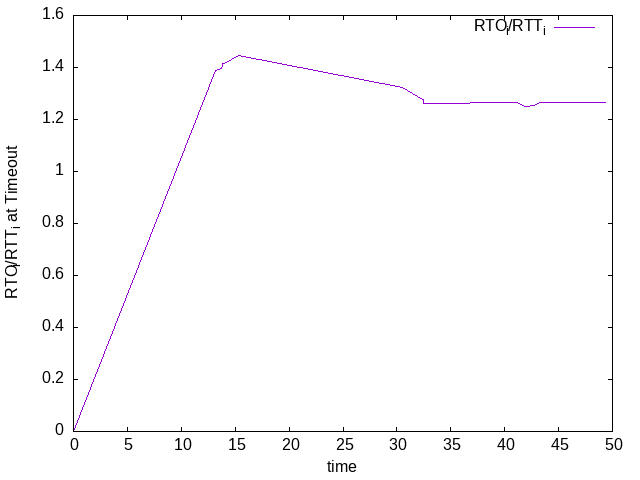
\includegraphics[height=.6\textwidth]{Pictures/rtt/175/m/mean_retransmission.png}
	\caption{Modified mean retransmission graph}
\end{figure}   

\newpage
\textbf{$RTO_i/RTT_i $ ratio}
\begin{figure}[H]
	\centering
	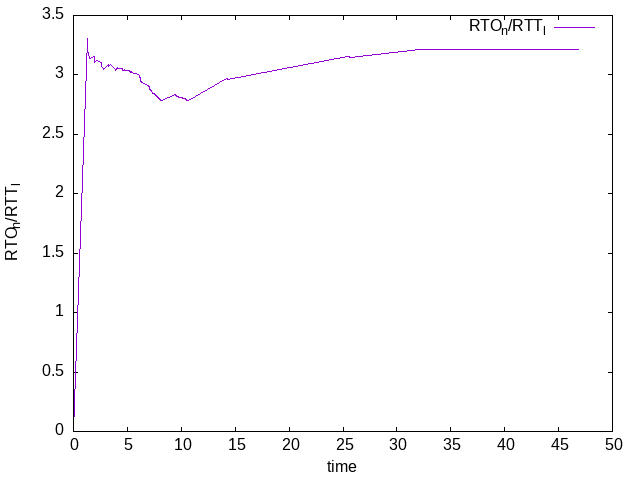
\includegraphics[height=0.6\textwidth]{Pictures/rtt/175/b/rto_by_rtt.png}
	\caption{Default rto/rtt graph}
\end{figure}   

\begin{figure}[H]
	\centering
	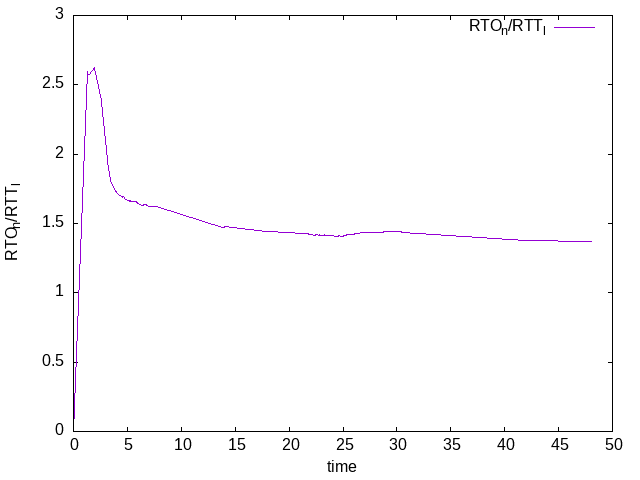
\includegraphics[height=0.6\textwidth]{Pictures/rtt/175/m/rto_by_rtt.png}
	\caption{Modified rto/rtt graph}
\end{figure}   

\newpage
\textbf{Congestion Window}
\begin{figure}[H]
	\centering
	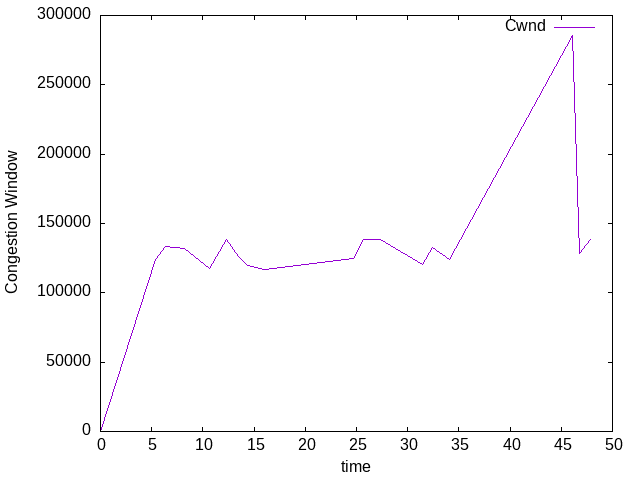
\includegraphics[height=0.6\textwidth]{Pictures/rtt/175/b/cwnd_graph.png}
	\caption{Default cwnd graph}
\end{figure}   

\begin{figure}[H]
	\centering
	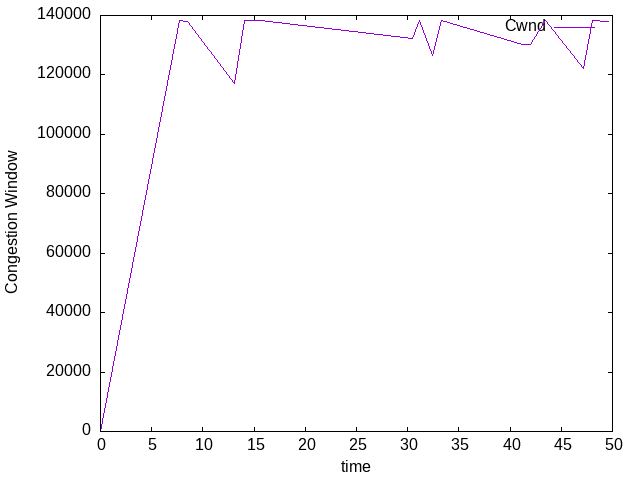
\includegraphics[height=0.6\textwidth]{Pictures/rtt/175/m/cwnd_graph.png}
	\caption{Modified cwnd graph}
\end{figure}   

\newpage
\textbf{Slow Start Threshold}
\begin{figure}[H]
	\centering
	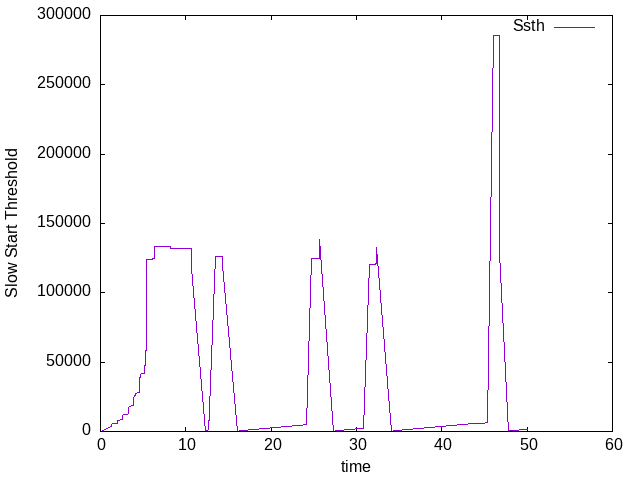
\includegraphics[height=0.6\textwidth]{Pictures/rtt/175/b/ssth_graph.png}
	\caption{Default ssth graph}
\end{figure}   


\begin{figure}[H]
	\centering
	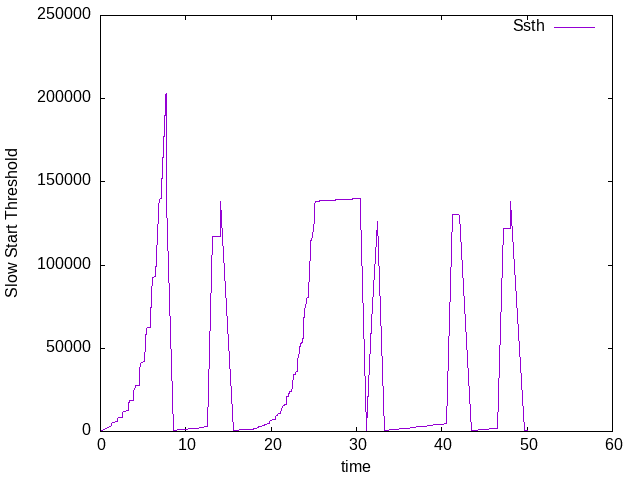
\includegraphics[height=0.6\textwidth]{Pictures/rtt/175/m/ssth_graph.png}
	\caption{Modified ssth graph}
\end{figure}   


%task A
\newpage
\subsection{Graphs of 802.11 and 802.15.4 protocol} 
\subsubsection{802.11 highrate static network}
\textbf{Network Topology Recap}

\begin{itemize}
	
	\item{\textbf{Propagation Model} ConstantSpeedPropagationDelayModel}
	\item{\textbf{Propagation Loss Model} RangePropagationLossModel}
	\item{\textbf{Mac}] AdhocWifiMac}
	\item{\textbf{Mac Standard} WIFI\_STANDARD\_80211b}
	\item{\textbf{Routing Protocol} AODV}
	\item{\textbf{Application Layer} OnoffHelper/ns3::UdpSocketFactory}
	\item{\textbf{Mobility Model} ConstantPositionMobilityModel}
	
\end{itemize}

\newpage
\vspace*{\fill}
\begin{center}
	\Large{Varying Number of Nodes}
\end{center}
\vspace*{\fill}


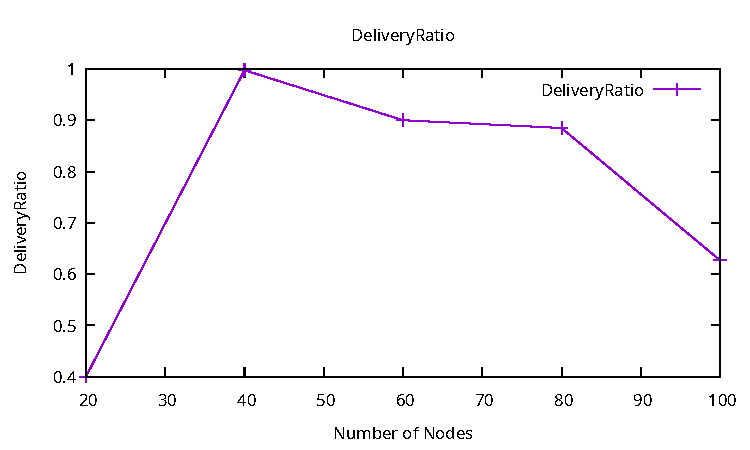
\includepdf[pages={1}]{11/n/dl.pdf}
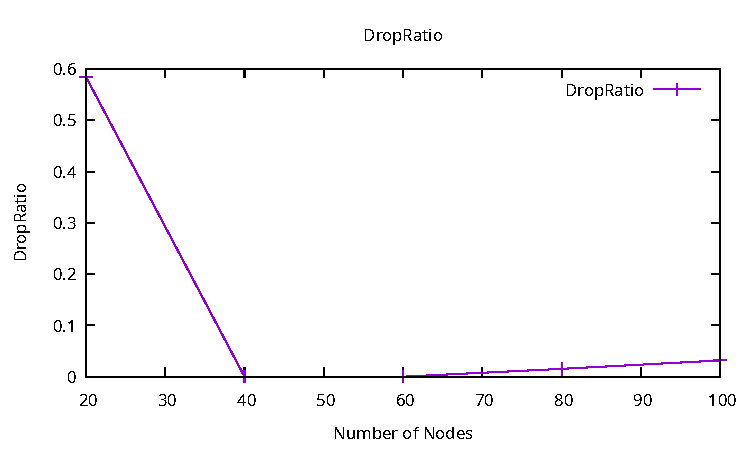
\includepdf[pages={1}]{11/n/dr.pdf}
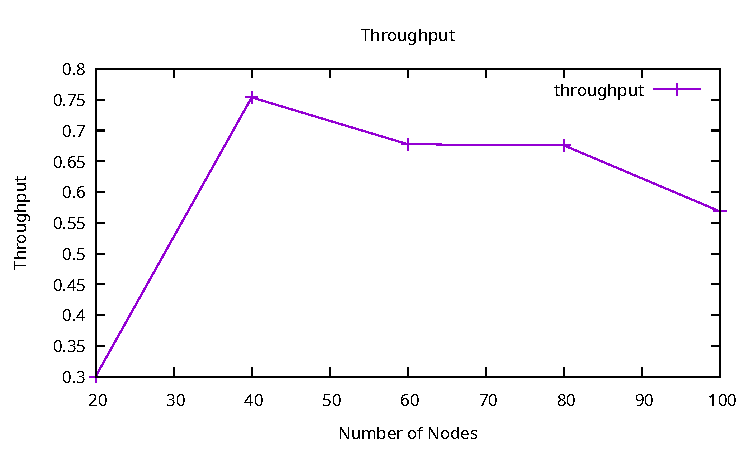
\includepdf[pages={1}]{11/n/t.pdf}
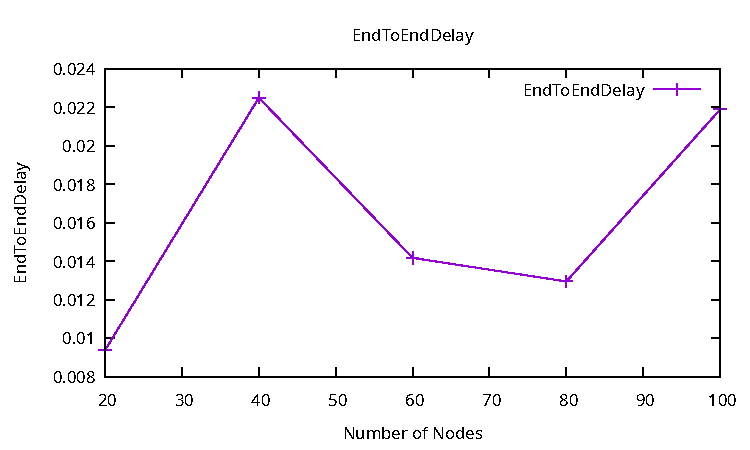
\includepdf[pages={1}]{11/n/e.pdf}


\vspace*{\fill}
\begin{center}
	\Large{Varying Coverage Area}
\end{center}
\vspace*{\fill}

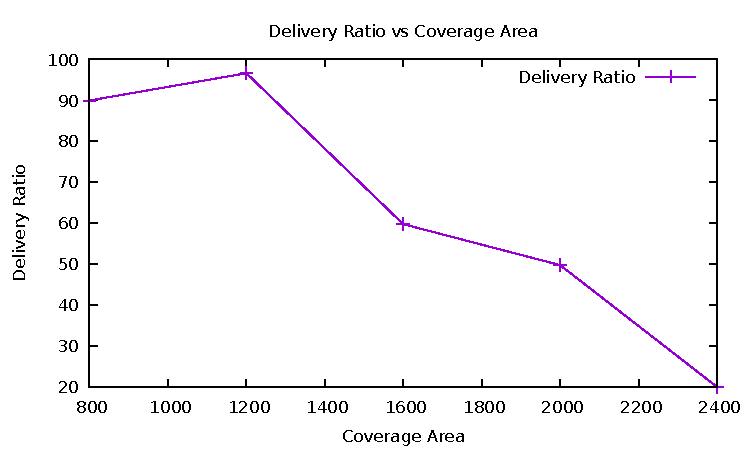
\includepdf[pages={1}]{11/c/dl.pdf}
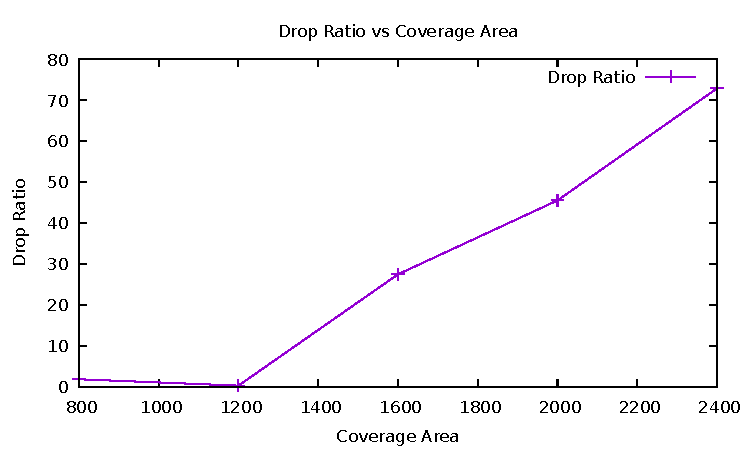
\includepdf[pages={1}]{11/c/dr.pdf}
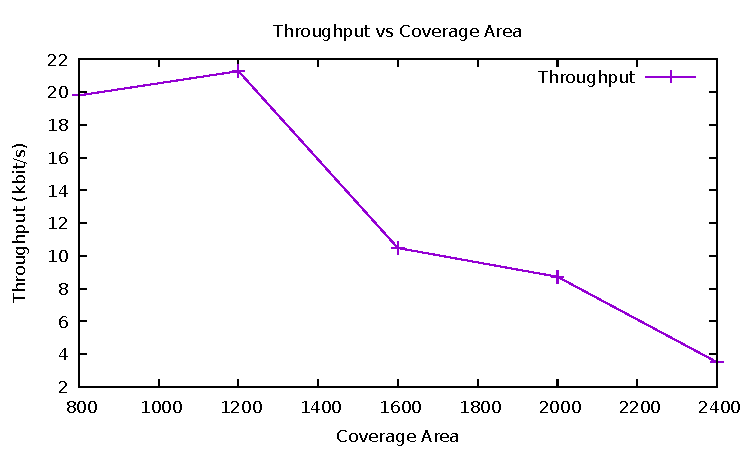
\includepdf[pages={1}]{11/c/t.pdf}
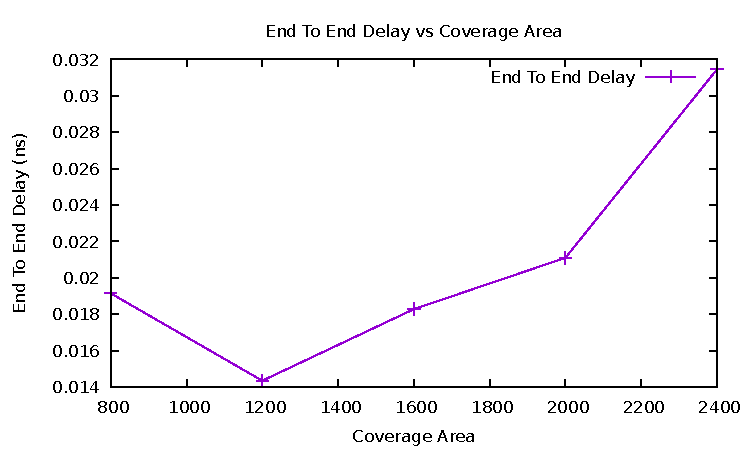
\includepdf[pages={1}]{11/c/e.pdf}

\vspace*{\fill}
\begin{center}
	\Large{Varying Number of Flows}
\end{center}
\vspace*{\fill}

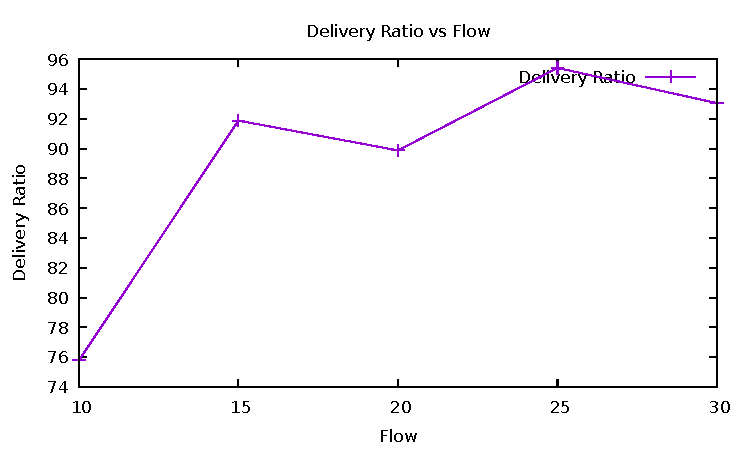
\includepdf[pages={1}]{11/f/dl.pdf}
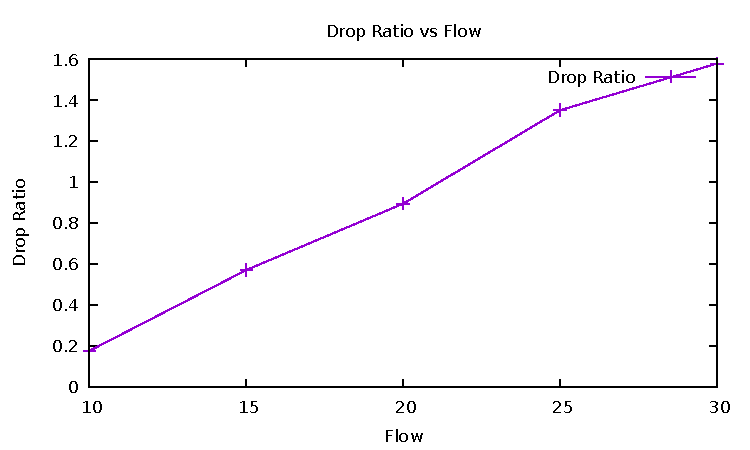
\includepdf[pages={1}]{11/f/dr.pdf}
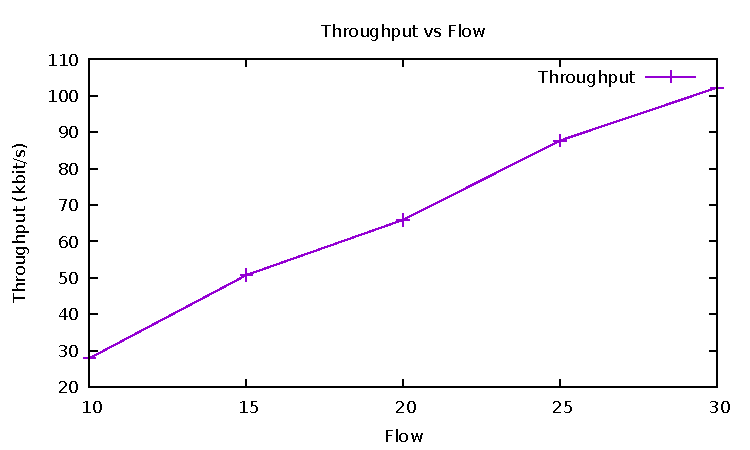
\includepdf[pages={1}]{11/f/t.pdf}
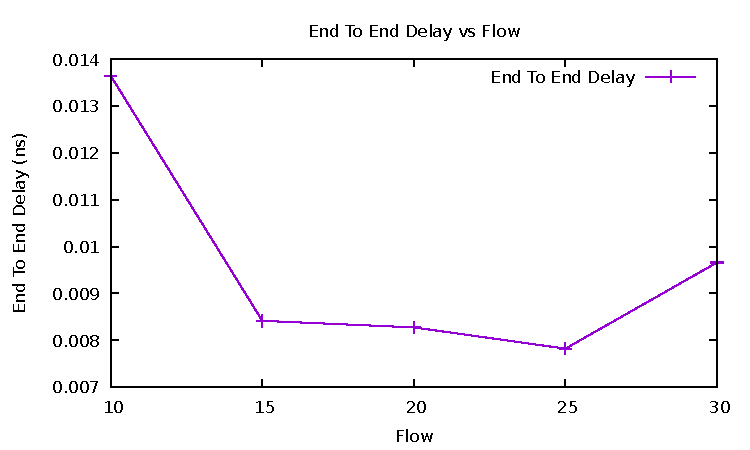
\includepdf[pages={1}]{11/f/e.pdf}

\vspace*{\fill}
\begin{center}
	\Large{Varying Number of Packets/Second}
\end{center}
\vspace*{\fill}

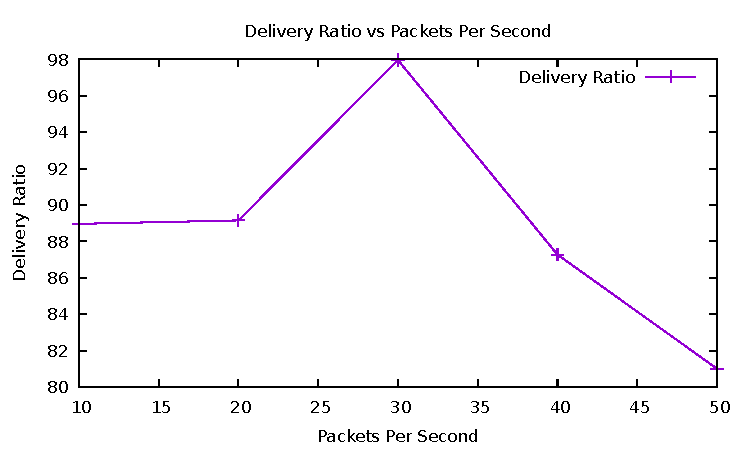
\includepdf[pages={1}]{11/p/dl.pdf}
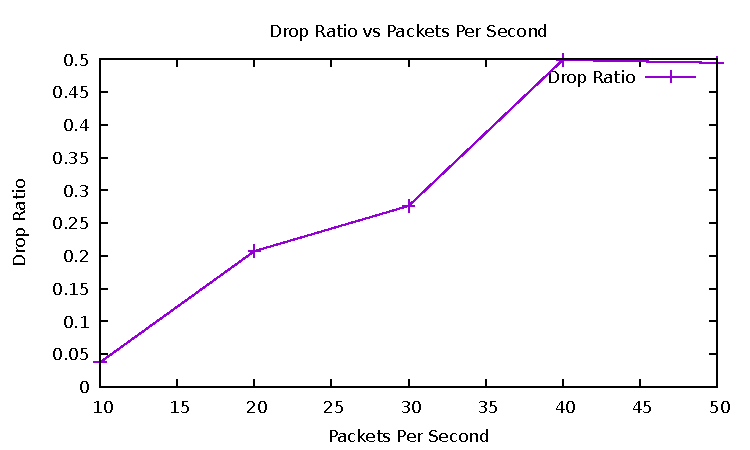
\includepdf[pages={1}]{11/p/dr.pdf}
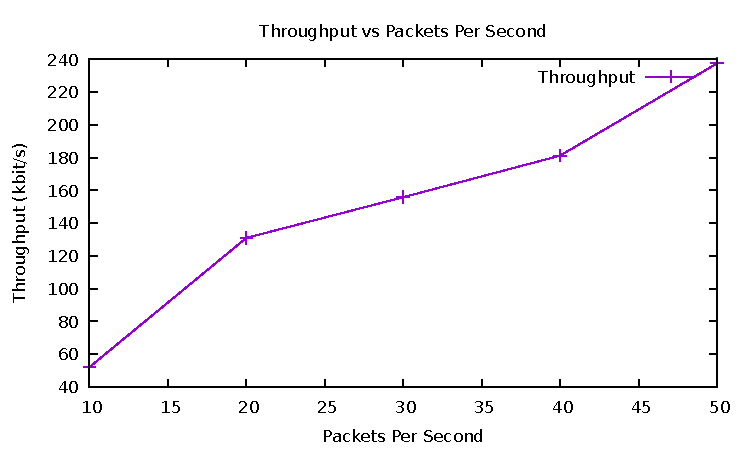
\includepdf[pages={1}]{11/p/t.pdf}
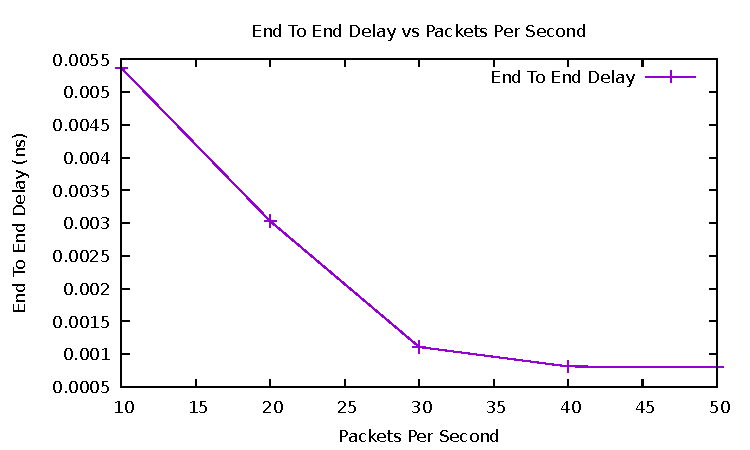
\includepdf[pages={1}]{11/p/e.pdf}


\subsubsection{802.15.4 lowrate static network}

\textbf{Network Topology Recap}

\begin{itemize}
	
	\item{\textbf{Propagation Loss Model} RangePropagationLossModel}
	\item{\textbf{Channel} LrwpanHelper}
	\item{Used \textbf{6LoWPAN} group that allows IPv6 packets to be sent and received over
		IEEE 802.15.4 based networks}
	\item{\textbf{Routing Protocol} Default Global Routing}
	\item{\textbf{Application Layer} OnoffHelper/ns3::UdpSocketFactory}
	\item{\textbf{Mobility Model} ConstantPositionMobilityModel}
	
\end{itemize}

\newpage

\vspace*{\fill}
\begin{center}
	\Large{Varying Number of Nodes}
\end{center}
\vspace*{\fill}

\newpage

\includepdf[pages={1}]{15/n/dl.pdf}
\includepdf[pages={1}]{15/n/dr.pdf}
\includepdf[pages={1}]{15/n/t.pdf}
\includepdf[pages={1}]{15/n/e.pdf}


\vspace*{\fill}
\begin{center}
	\Large{Varying Coverage Area}
\end{center}
\vspace*{\fill}

\includepdf[pages={1}]{15/c/dl.pdf}
\includepdf[pages={1}]{15/c/dr.pdf}
\includepdf[pages={1}]{15/c/t.pdf}
\includepdf[pages={1}]{15/c/e.pdf}

\vspace*{\fill}
\begin{center}
	\Large{Varying Number of Flows}
\end{center}
\vspace*{\fill}

\includepdf[pages={1}]{15/f/dl.pdf}
\includepdf[pages={1}]{15/f/dr.pdf}
\includepdf[pages={1}]{15/f/t.pdf}
\includepdf[pages={1}]{15/f/e.pdf}

\vspace*{\fill}
\begin{center}
	\Large{Varying Number of Packets/Second}
\end{center}
\vspace*{\fill}

\includepdf[pages={1}]{15/p/dl.pdf}
\includepdf[pages={1}]{15/p/dr.pdf}
\includepdf[pages={1}]{15/p/t.pdf}
\includepdf[pages={1}]{15/p/e.pdf}


\section{Summary}

\subsection{Explanation of Results found in 802.11 static network}

	\textbf{\textcolor{blue}{Varying Number of Nodes}}
  \begin{itemize}
  	\item \textbf{Throughput} : Decreases as increase of node congesting the network flow more
  	\item \textbf{End-to-End Delay} : Increases because of more congested network
  	\item \textbf{Delivery Ratio} : Decreases with increase of more nodes congested in same network
  	\item \textbf{Drop Ratio} : Starts to increase a little bit because of network congestion.
  \end{itemize}


   \textbf{\textcolor{blue}{Varying Number of Flows}}
	\begin{itemize}
	\item \textbf{Throughput} : Increases due to more flow in the network
	\item \textbf{End-to-End Delay} :Decreases due to more flow in the network
	\item \textbf{Delivery Ratio} : Shows a trend of decrease with increasing flows
	\item \textbf{Drop Ratio} : Increases because of network congestion.
	\end{itemize}

 \textbf{\textcolor{blue}{Varying Number of Packets/Second}}
\begin{itemize}
	\item \textbf{Throughput} : Increases due to more packets flowing in the network.
	\item \textbf{End-to-End Delay} :Decreases due to more packets flowing in the network.
	\item \textbf{Delivery Ratio} : Shows a trend of decrease with more packets flowing. 
	\item \textbf{Drop Ratio} : Increases because of network congestion due to more packet flow.
\end{itemize}

 \textbf{\textcolor{blue}{Varying Number of Coverage Area}}
\begin{itemize}
	\item \textbf{Throughput} : Decreases due to large area and randomness in the network.
	\item \textbf{End-to-End Delay} :Increases due to larger network.
	\item \textbf{Delivery Ratio} : Shows a trend of decrease larger area network.
	\item \textbf{Drop Ratio} : Increases because of randomness in a large network.
\end{itemize}


\newpage


\subsection{Explanation of Results found in 802.15.4 static network}

\textbf{\textcolor{blue}{Varying Number of Nodes}}
\begin{itemize}
	\item \textbf{Throughput} :No common pattern of monotonic increase or decrease shown.
	\item \textbf{End-to-End Delay} : Increases because of more congested network
	\item \textbf{Delivery Ratio} : Decreases with increase of more nodes congested in same network
	\item \textbf{Drop Ratio} : Starts to increase a little bit because of network congestion.
\end{itemize}


\textbf{\textcolor{blue}{Varying Number of Flows}}
\begin{itemize}
	\item \textbf{Throughput} : Increases due to more flow in the network
	\item \textbf{End-to-End Delay} :Increases due to more flow and congestion in the network
	\item \textbf{Delivery Ratio} : Shows a trend of decrease with increasing flows
	\item \textbf{Drop Ratio} : Increases because of network congestion.
\end{itemize}

\textbf{\textcolor{blue}{Varying Number of Packets/Second}}
\begin{itemize}
	\item \textbf{Throughput} : Increases due to more packets flowing in the network.
	\item \textbf{End-to-End Delay} :Decreases due to more packets flowing in the network.
	\item \textbf{Delivery Ratio} : Shows a trend of decrease with more packets flowing. 
	\item \textbf{Drop Ratio} : Increases because of network congestion due to more packet flow.
\end{itemize}

\textbf{\textcolor{blue}{Varying Number of Coverage Area}}
\begin{itemize}
	\item \textbf{Throughput} : Decreases due to large area and randomness in the network.
	\item \textbf{End-to-End Delay} :Increases due to larger network.
	\item \textbf{Delivery Ratio} : Shows a trend of decrease larger area network.
	\item \textbf{Drop Ratio} : Increases because of randomness in a large network.
\end{itemize}
    
\newpage

\subsection{Explanation of Performance Metrics Result in RTT/RTO modification algorithm}

The PeakHopper paper calculated three performance metrics and I analysed two of them in my implementation.From the mean retransmission graph , it's seen that modified algorithm provides a lower mean retransmission than default Jacobson's implementation.It was expected because a lower mean indicates that retransmission timer follows a narrow waiting time and a higher mean indicates to a longer waiting time.\\

Another metric,known as the mean of RTO\_N/RTT\_L where  RTO\_N is the newly calculated RTO
and RTT\_L is the last RTT sample prior to the RTO
update. We then calculated P as the mean value of this
fraction over an entire simulation run.This mean is found to be lower in modified algorithm than in default implementation which is expected too.A retransmission timer with lower mean of this ratios is expected to perform better.\\

From these mean calculations , an explanation of those sudden rise of RTO can be given.Since a mean over the entire simulation run is taken and those spikes are very transient , therefore , they don't contribute much to the performance metrics calculated in the paper.Thus , the implementation appears to perform in line with our expectation.  
\end{document}
